% Chapter Template

\chapter{Proposed Approach} % Main chapter title

\label{chapter4} % Change X to a consecutive number; for referencing this chapter elsewhere, use \ref{ChapterX}

\lhead{Chapter 4. \emph{Proposed Approach}} 

This section gives a detailed description of the implemented tracking system. Initially, giving an overview of the whole system and the basic functional blocks. Then, explaining implementation details of the different parts.

\section{The Tracking Loop}

Initially,  we explain the necessary building blocks of an object tracking system.

\section{Tracking system overview}

In order to tackle all the problems stated in the previous section, this tracking approach is separated into different modules.

\subsection{Basic overview}

Generic single-object tracking could be defined as the localization of an object through a video sequence. It is generic because the system is able to track any kind of object (faces, cars, etc.), and is single because the system will track just one object and not many at the same time. The proposed approach in this thesis is shown in \ref{fig::diagram}. Initially, our method starts with a pool of trackers $T = {t_1, t_2, ..., t_n}$ and input data $\mathrm{x}$. This input corresponds to the initial rectangular box for an object in a sequence. All trackers are initalized and an updateable object model is created. Then, on each frame, our method runs and groups all trackers results by position into a set of clusters $C = {c_1, c_2, ..., c_m}$. Also, we obtain a similarity measure which compares an actually tracking result patch to the current object model. The output should be the probabilities of similarity between the object model and each tracker result in that frame. Using clustering information, the system can select between the winner cluster $c*$ which has the highest number of members, or the cluster with highest similarity measure. the others clusters are considered outliers and are reinitialized each 15 frames.

\begin{figure}[t!]
	\centering
		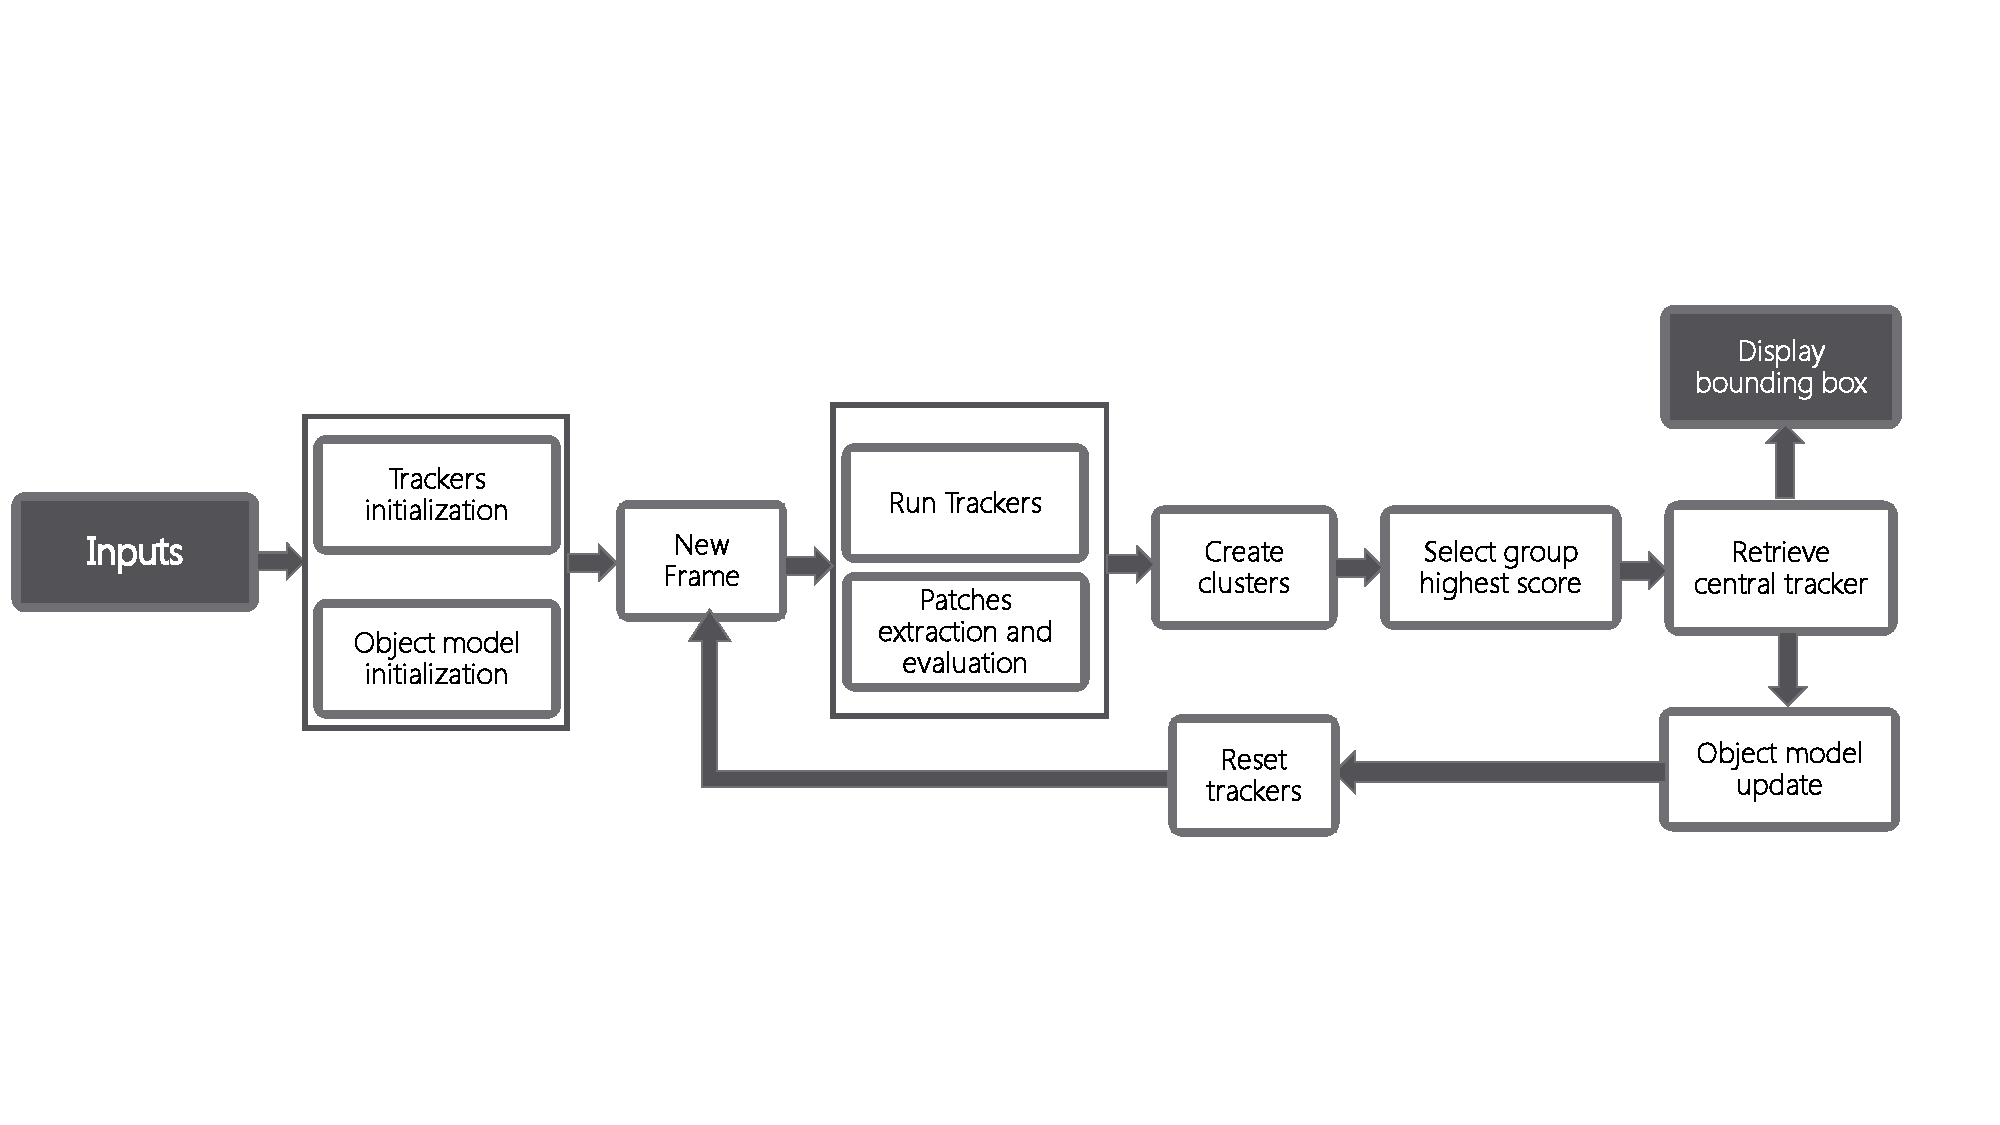
\includegraphics[width=1\linewidth, trim= 0cm 3cm 1cm 4cm, clip=true]{Figures/block_diagram.pdf}
	\caption{General schema for generic single-object tracking proposal.}
	\label{fig::diagram}
\end{figure}

\subsection{Trackers clustering}

Cluster analysis is the formal study of algorithms and methods for grouping, or classifying objects. These objects are described as a set of measurements or by relationships between the object and other objects. A \textit{cluster} is comprised of a number of similar objects collected or group together. Other authors define a cluster as a set of entities which are alike, and entities from different clusters are not alike, or "A cluster is an aggregation of points in the test space such that the \textit{distance} between any two points in the cluster is less than the distance between any point in the cluster and any point not in it". This theory is taken from \textbf{Jane and Dubes.}

Cluster analysis is the process of classifying objects into subsets that have meaning in the context of a particular problem. The objects are thereby organized into an efficient representation that characterizes the data. Clustering methods require that an index of proximity, or alikeness, or affinity, or association be established between pairs or patterns. A \textit{proximity matrix} $|d(i, j)|$ accumulates the pairwise indices of proximity in a matrix in which each row and column represents a pattern. Diagonal entries of a proximity matrix are ignored since all paterns are assumed to have the same degree of proximity with themselves. Also it is assmed that all proximity matrices are symmetric, so all pairs of objects have the same proximity index, independent of the order in which they are written.

A proximity index is either a \textit{similarity} or a \textit{dissimilarity}. The more the \textit{i}th and \textit{j}th objects are similar one another, the larger a similarity index and the dissimilarity index are.

Previous works show the common approach of data fusion using majority voting. The authors in \cite{Bailer2013} applied this method using a threshold parameter that defines if two result boxes vote for the same position. However, in \cite{Bailer2014}, the authors proved that this approach is sequence dependent. Instead, they settle the idea of attraction fields. We base our approach using the idea of clustering position. On a new frame, each tracker will give a rectangular box of where the object might be. Using this information, we are able to form groups of trackers that have similar positions. For each tracker result, we calculate the distance between its position and the rest of trackers running. The distance $d$ between two boxes $b$ and $c$ is computed as:

\begin{equation}
\large
d(b,c) = 1 - \frac{b\bigcap c}{b\bigcup  c}
\end{equation}

\noindent Using all distances, we construct a symmetric $l \times l$ proximity matrix $D$. We take the proximities to be dissimilarities. This means that $d(i,i) = 0$ for all $i$. We use complete-link hierarchical agglomerative clustering to form groups of trackers. Trackers $t_1$ and $t_2$ are "related" if their dissimilarity is below some threshold $v$. CL merges clusters in order of proximity; the closest clusters will be merged first, and the furthest clusters will be merged last. At each merge, CL creates a \textit{reduced proximity matrix}, with one less row and column.
